\documentclass[UTF8,a4paper,11pt,fontset=fandol]{ctexart}
\usepackage[left=24mm,right=24mm,top=23mm,bottom=24mm]{geometry}
\usepackage{booktabs,longtable,tabularx,array,graphicx,xcolor,amsmath,amssymb,amsthm,fancyhdr,hyperref,enumitem}
\usepackage[normalem]{ulem}
\hypersetup{colorlinks=true,linkcolor=blue!50!black,urlcolor=blue!60!black,citecolor=blue!50!black}
\definecolor{lightblue}{RGB}{235,242,250}
\definecolor{lightred}{RGB}{253,238,238}
\definecolor{lightyellow}{RGB}{255,250,225}
\definecolor{deepred}{RGB}{160,30,30}
\newcolumntype{R}{>{\raggedleft\arraybackslash}p{2.1cm}}
\setlength{\parindent}{2em}\setlength{\parskip}{0.35em}
\pagestyle{fancy}\setlength{\headheight}{14pt}\fancyhf{}
\lhead{CGM（2005）复现差异根因溯源}\rhead{433 vs 221.5}\cfoot{\thepage}
\newcommand{\su}{\sigma_u^2}
\newcommand{\suDP}{\sigma_{u,\mathrm{DP}}^{2}}
\newcommand{\se}{\sigma_\varepsilon^2}
\title{\bfseries Cocco--Gomes--Maenhout（2005）\\复现差异根因溯源报告\\[4pt]
\large 为什么退休财富是 433 千美元而不是 221.5 千美元}
\author{独立复核：从论文方程重写求解器 \(+\) 出版图的矢量数字化 \(+\) 消融实验}
\date{2026 年 9 月 11 日}
\begin{document}\maketitle

\begin{center}
\colorbox{lightblue}{\parbox{0.93\textwidth}{
\textbf{结论先行。}（1）433 千美元不是任何一版程序的书写错误：本次从论文方程重新独立写出的 EGM 求解器给出 \textbf{434.1}，与既有 Matlab 改造版的 433.4 相差 0.2\%，并通过机器精度的解析反例与网格收敛检验。（2）论文图 2C 的\textbf{退休段}（65 岁）消费政策被复现到 RMSE \(=0.14\) 千美元，说明收益、偏好、死亡率、退休接口、终值条件与算法全部无误。（3）论文图 2C 的\textbf{工作年段}（20、35 岁）出现约 8.5 千美元（约 40\%）的系统性偏离，偏离的量级与符号恰好等于永久收入冲击 \(\sigma_u\) 在 Euler 方程中产生的\textbf{预防性/对冲项}。（4）把这一项关掉以后，图 2C 三个年龄的 RMSE 从 \(8.6/8.4/0.14\) 降到 \(0.12/0.20/0.14\)，图 3A 的 65 岁财富从 435 降到 206--222（论文 221.5），消费收入比 \(C/Y(25)\) 从 0.716 升到 0.965--0.968（论文 0.969）。单参数识别给出 \(\suDP\approx 5\times10^{-4}\) 时 \(W_{65}=221.5\)，与论文的 221.476 重合。（5）因此，\textbf{“原 Matlab 求解环节有 bug”这一说法应当撤回}；正确的表述是：论文式（2）--（5）写出的模型与出版图表不能被同一套永久收入风险处理同时匹配。（6）表 6 是\textbf{另一个独立的、仍未解决}的差异：能匹配图 2／图 3 的参数会让表 6 的损失低一个数量级，而能匹配表 6“近似规则”一列所需的参数会把 \(W_{65}\) 推到 348。}}
\end{center}

\tableofcontents\newpage

\section{任务、基准与本文的判定标准}

\subsection{要回答的问题}
前几轮工作留下的核心悬案是：严格按 CGM（2005）论文实现的求解器给出 65 岁平均金融财富约 \textbf{433 千美元}，而论文图 3A 给出约 \textbf{221.5 千美元}；同时论文表 6 的福利损失也难以对上。围绕这一差距已经出现过互相矛盾的判断——一套说法是“原来的 Matlab 在动态规划求解环节有 bug”，另一套说法是“Python 版本在消费约束、冲击相关性、延续价值上有实现错误”。本报告的目的是把这一差距\textbf{定位到具体的模型项或代码项}，而不是再给出一版数字。

\subsection{判定标准}
本报告不接受“谁的数字更接近论文，谁就更正确”作为判据。采用的判据是三条互相独立的证据：
\begin{enumerate}[leftmargin=2.2em,itemsep=1pt]
\item \textbf{独立重写}:从论文的 Bellman 方程、Euler 方程与预算约束重新写一个求解器，若与既有实现一致，则说明该结果不是书写疏漏，而是该模型设定的必然输出。
\item \textbf{出版图的矢量数字化}:不依赖从图片上“目测读数”，而是直接从论文 PDF 的矢量图层提取曲线坐标（第 \ref{sec:digit} 节）。这样得到的基准精度约为千分之一千美元。
\item \textbf{消融实验}:把每一个可疑设定做成开关，逐个打开/关闭，观察哪一个开关能把结果从 433 移动到 221.5，同时不破坏其他已经被匹配的曲线。
\end{enumerate}

\subsection{论文基准的精确口径}
\label{sec:digit}
论文给出的是图片而不是数据文件，因此必须先建立可比的数值基准。本次使用 PyMuPDF 读取 \texttt{cgm.pdf} 的\emph{绘图指令}（该 PDF 的图形是矢量而非位图），按坐标轴刻度做线性标定，再按线宽把折线链成曲线。关键标定值如下（单位：PDF 点）：

\begin{table}[htbp]\centering\small
\caption{图 2 与图 11 的坐标标定（均取自页面文字层的刻度标签）}\vspace{-2pt}
\begin{tabular}{@{}lll@{}}\toprule
图 & 横轴 & 纵轴\\\midrule
图 2B（\(\alpha(x,t)\)）& 现金 \(0\!\to\!300\) & 刻度 \(0,0.2,\ldots,1.0\)\\
图 2C（\(C(x,t)\)）& 现金 \(0\!\to\!300\) & 刻度 \(0,10,\ldots,50\)\\
图 11（规则 \(\alpha_t\)）& 年龄 \(20\!\to\!95\) & 刻度 \(0,0.2,\ldots,1.0\)\\\bottomrule
\end{tabular}
\end{table}

由此读出、并在本报告中作为\textbf{唯一}比较基准的论文数值：

\begin{table}[htbp]\centering\small
\caption{从论文图 3 矢量图层提取的生命周期基准（千美元，1992 年美元）}\vspace{-2pt}
\begin{tabular}{@{}lrrrrrrrr@{}}\toprule
年龄 & 20 & 25 & 30 & 40 & 50 & 60 & 65 & 66\\\midrule
收入 & 16.45 & 21.71 & 26.98 & 32.91 & 33.57 & 32.91 & 32.36 & 22.16\\
财富 & --- & 10.33 & 18.32 & 56.50 & 125.14 & 192.82 & \textbf{221.48} & 215.57\\
消费 & --- & 21.03 & 26.31 & 30.93 & 32.91 & 34.89 & 35.55 & 35.55\\
股票份额 & 0.963 & 1.000 & 1.000 & 0.989 & 0.846 & 0.604 & \textbf{0.499} & 0.504\\\bottomrule
\end{tabular}
\end{table}

两处对本文判定至关重要的读法：
\begin{itemize}[leftmargin=1.6em,itemsep=1pt]
\item 收入在 65 岁为 32.36、在 66 岁骤降到 22.16，二者之比 \(22.16/32.36=0.685\)，与高中组退休替代率 \(\lambda=0.68212\) 吻合。因此论文的“最后一个工作年”是 \textbf{65 岁}，退休收入从 \textbf{66 岁}开始。
\item 把论文自己的收入、消费、股票份额路径代入预算恒等式 \(W_{t+1}=(W_t+Y_t-C_t)(R_f+\alpha_t\mu)\)，得到 65 岁财富 \textbf{194.1}，与图上 221.5 相差 12\%（差额来自 \(\mathrm{Cov}(S_t,R_{p,t+1})\) 与数字化误差）。这说明\textbf{论文图 3 自身是自洽的}，不能用“图上读数有误”来解释差距。
\end{itemize}

\section{参数对照：我们是否严格采用了论文参数}

\subsection{论文参数}
高中组基准参数来自论文表 1（回归常数 2.7004）、表 2（年龄多项式，工作期到 65 岁）、表 3（方差分解）与表 4（偏好与市场）。确定性收入函数为
\begin{equation}
F(a)=\exp\big[(2.700381-2.170042)+0.16818\,a-\tfrac{0.0323371}{10}a^2+\tfrac{0.0019704}{100}a^3\big],
\end{equation}
其中 \(-2.170042\) 是表 2 的多项式常数项、\(2.700381\) 是表 1 的回归常数项，二者相加得 0.530339。这一点常被误读：若只取表 2 的 \(-2.1700\)，20 岁收入会变成 1.96 千美元而不是约 16 千美元。

\subsection{逐项对照}
表 \ref{tab:params} 把论文设定、Gomes 通用模板默认值、本次独立实现、既有 Matlab 改造实现与 DeepSeek Python 实现放在一起。

\begin{longtable}{@{}p{0.205\textwidth}p{0.145\textwidth}p{0.135\textwidth}p{0.115\textwidth}p{0.115\textwidth}p{0.135\textwidth}@{}}
\caption{参数与实现对照}\label{tab:params}\\\toprule
项目 & 论文 CGM(2005) & 模板默认 & 本次实现 & Matlab 改造版 & DeepSeek Python\\\midrule
\endfirsthead\toprule
项目 & 论文 & 模板默认 & 本次实现 & Matlab 版 & Python 版\\\midrule\endhead
风险厌恶 \(\gamma\) & 10（表 4） & 10 & 10 & 10 & 10\\
年贴现因子 \(\delta\) & 0.96（表 4） & \textbf{0.97} & 0.96 & 0.96 & 0.96\\
无风险总收益 \(R_f\) & 1.02（表 4） & \textbf{1.015} & 1.02 & 1.02 & 1.02\\
股票超额收益 \(\mu\) & 0.04（表 4） & 0.04 & 0.04 & 0.04 & 0.04\\
股票收益标准差 & 0.157（表 4） & \textbf{0.20} & 0.157 & 0.157 & 0.157\\
暂时冲击方差 \(\se\) & 0.0738（表 3/4） & \textbf{0.01} & 0.0738 & 0.0738 & 0.0738\\
永久冲击方差 \(\su\) & 0.0106（表 3/4） & \textbf{0.01} & 0.0106 & 0.0106 & 0.0106\\
收入--股票相关系数 & 0（表 4） & 0 & 0 & 0 & 0\\
退休 & 65 最后工作年 & \(t_r=66\) & 65 末/66 首 & 65 末/66 首 & 65 末/66 首\\
退休替代率 \(\lambda\) & 0.68212（表 2） & 0.68212 & 0.68212 & 0.68212 & 0.68212\\
遗产动机 & 0 & 可扩展 & 0 & 0 & 0\\
偏好形式 & 时间可加 CRRA & \textbf{Epstein--Zin，EIS 0.5} & CRRA & CRRA & CRRA\\
\bottomrule
\end{longtable}

结论：\textbf{所有标量参数在三套实现与论文之间一致}（模板默认值不同之处已被替换；模板的 Epstein--Zin 形式也已被换成论文的 CRRA）。也就是说，\textbf{差异不出在参数取值，而出在公式实现}——具体地，出在永久收入冲击进入延续价值的那一项。

\subsection{被明确记录的实现选择}
以下四项目论文正文没有给出可核对的代码，属于实现自由度，本次统一固化并逐项检验过敏感性：
（i）初始金融财富为 0；
（ii）初始永久收入 \(\nu_{20}=0\)（即 \(P_{20}=F(20)\)）；
（iii）模拟 20\,000 个家庭、反向冲击对（antithetic）减方差；
（iv）\(\nu\) 为对数随机游走，因此水平永久收入含有 \(\exp(\su/2)\) 的漂移。第（iv）项不是可选项：只有保留该漂移，模拟的平均收入曲线才会在 50 岁达到论文的 33.6 千美元（本次模型 33.6，论文 33.57）。

\section{复现结果一：433 不是实现错误}

\subsection{两个独立实现给出同一答案}
本次按论文方程从头写出的 EGM 求解器（\texttt{ref\_cgm.py}）与既有 Matlab 改造求解器（\texttt{cgm\_solve.m}）在两套完全不同的算法框架下给出：

\begin{table}[htbp]\centering\small
\caption{两套独立实现的输出对照（模拟规模 20\,000，同一随机种子不可共享）}\vspace{-2pt}
\begin{tabular}{@{}lrrrr@{}}\toprule
& 65 岁财富 & 65 岁消费 & 65 岁股票份额 & 25 岁消费/收入\\\midrule
Matlab 改造版（网格 EGM，801 点，\(9^3\) 求积） & 433.4 & 45.9 & 0.3652 & 0.717\\
本次独立实现（EGM，401 点，\(7^3\) 求积） & \textbf{434.1} & 46.08 & 0.3652 & 0.716\\
论文图 3 & 221.5 & 35.55 & 0.499 & 0.969\\\bottomrule
\end{tabular}
\end{table}

65 岁股票份额在两种实现之间吻合到小数点后四位。两套代码在网格大小、求积阶数、插值方式、编程语言、循环结构上都不同，却给出同一答案，因此\textbf{不存在“某一行写错”的解释空间}。

\subsection{求解器自身的验收}
\begin{table}[htbp]\centering\small
\caption{本次实现的数值验收}\vspace{-2pt}
\begin{tabular}{@{}p{0.40\textwidth}p{0.50\textwidth}@{}}\toprule
检验 & 结果\\\midrule
两期解析反例（99 岁，无收益风险） & \(c^*(x)=\frac{R_fx+\lambda}{R_f+(\beta p R_f)^{1/\gamma}}\)，
\(x=1,\ 2,\ 5\) 处误差 \(<10^{-15}\)\\
Euler 方程回代 & 抽样年龄与储蓄点上的相对误差 \(<10^{-15}\)（构造性恒等式）\\
网格收敛 & \(n_q=5,7,9\)，\(n_a=301,401,801,1601\)，\(W_{65}\) 稳定在 176.5--176.7（无永久风险设定）\\
冲击独立性 & 永久、暂时、收益三个创新使用独立求积维（\(9^3=729\) 点）\\
约束 & 消费不超现金（\(c\le x\)）、\(\alpha\in[0,1]\)、\(a\ge0\) 全部显式施加\\
\bottomrule
\end{tabular}
\end{table}

\subsection{代码级审计：既有 Matlab 改造实现}
逐行复核 \texttt{cgm\_solve.m} 与 \texttt{cgm\_simulate.m}，未发现会改变最优决策的错误。要点：
\begin{itemize}[leftmargin=1.6em,itemsep=1pt]
\item 三个创新使用独立求积维：永久冲击挂在 \texttt{zp}、暂时冲击挂在 \texttt{zt}、收益挂在 \texttt{zr}，联合权重为乘积，符合论文表 4 的 \(\rho=0\)。
\item Euler 方程使用 \((G\,c')^{-\gamma}\)，股票一阶条件使用完整的包络条件 \(\mathbb{E}[(Gc')^{-\gamma}(R-R_f)]=0\)，与第 \ref{sec:appendix} 节的推导一致。
\item 借款约束通过 EGM 端点 \((x,c)=(0,0)\) 与 \((c(a{=}0),c(a{=}0))\) 之间的线性插值实现为 \(c=x\)，是正确的约束区处理。
\item 终期条件 \(c_T=x_T\)、退休后 \(G=1,\ y=\lambda\)、\(\lambda\) 冻结在 \(P_{65}\)，均与式（5）一致。
\item 两处\textbf{真实但不改变结论的缺陷}应记录：（a）\texttt{cgm\_solve.m} 第 17 行以 “年龄 \(\ge 65\)” 进入退休分支，而 \texttt{cgm\_simulate.m} 第 18 行以 “年龄 \(\le 65\)” 保留工作收入，求解与模拟在 65 岁当年不一致（论文的 65 岁是最后一个工作年）；本次实现已统一为 65 岁工作、66 岁退休。（b）高现金区域 \(\alpha\) 政策的外插不稳（\(x\!\approx\!250\) 千美元处出现回弹），但该区域在模拟中不会被访问。
\end{itemize}

至此可以确认：\textbf{433 是论文式（2）--（5）加表 4 参数这一组设定的正确解}。问题因此转化为——论文的出版图是否出自这同一组设定？

\section{复现结果二：退休段政策函数被精确复现}

图 2C 是论文的消费政策函数 \(C(x,t)\)（水平值，千美元）。其中 65 岁一档完全落在退休期（不涉及永久收入风险）。本次实现与该曲线的对比：

\begin{table}[htbp]\centering\small
\caption{图 2C 65 岁消费政策：论文 vs 本次实现（千美元）}\vspace{-2pt}
\begin{tabular}{@{}lrrrrrrrrrrrr@{}}\toprule
现金 \(x\) & 10 & 15 & 20 & 25 & 30 & 40 & 50 & 75 & 100 & 150 & 200 & 250\\\midrule
论文图 2C & 10.0 & 15.3 & 17.5 & 18.1 & 18.6 & 19.3 & 20.1 & 21.8 & 23.3 & 26.0 & 28.6 & 31.1\\
本次实现 & 10.0 & 15.0 & 17.4 & 17.9 & 18.4 & 19.2 & 20.0 & 21.7 & 23.2 & 25.9 & 28.5 & 30.9\\\midrule
\(c/x\) 论文 & 1.00 & 1.02 & 0.88 & 0.72 & 0.62 & 0.48 & 0.40 & 0.29 & 0.23 & 0.17 & 0.14 & 0.12\\
\(c/x\) 本次 & 1.00 & 1.00 & 0.87 & 0.72 & 0.61 & 0.48 & 0.40 & 0.29 & 0.23 & 0.17 & 0.14 & 0.12\\\bottomrule
\end{tabular}
\end{table}

RMSE 为 \textbf{0.14 千美元}（相对消费水平约 0.6\%）。这一条同时锁定了：CRRA 效用与 \(\gamma=10\)、\(\delta=0.96\)、\(R_f=1.02\)、\(\mu=0.04\)、\(\sigma=0.157\)、NCHS 生存概率表、退休收入 \(y=\lambda\) 的设定、终期条件、以及 EGM 与插值算法。凡是这些环节出错，都不可能同时对上 12 个现金水平上的 65 岁消费。

\section{复现结果三：工作年段出现系统性偏离}

同样的比较放到 20 岁与 35 岁（工作年段，永久收入风险起作用）：

\begin{table}[htbp]\centering\small
\caption{图 2C 20 岁消费政策：论文 vs 两类实现（千美元）}\vspace{-2pt}
\begin{tabular}{@{}lrrrrrrrrrrrr@{}}\toprule
现金 \(x\) & 10 & 15 & 20 & 25 & 30 & 40 & 50 & 75 & 100 & 150 & 200 & 250\\\midrule
论文图 2C & 10.0 & 13.7 & 15.6 & 17.3 & 18.3 & 20.4 & 21.8 & 24.8 & 27.1 & 29.8 & 32.0 & 33.8\\
本次实现，\(\su=0.0106\) & 10.0 & 13.5 & 15.7 & 17.2 & 18.5 & 20.4 & 22.0 & 24.9 & 27.0 & 29.9 & 32.1 & 33.9\\
本次实现，\(\su=0\) & 10.0 & 13.5 & 15.7 & 17.2 & 18.5 & 20.4 & 22.0 & 24.9 & 27.0 & 29.9 & 32.1 & 33.9\\\bottomrule
\end{tabular}
\end{table}

表 \ref{tab:fig2c-rmse} 汇总了三个年龄上的 RMSE。规律非常清楚：\textbf{退休段完全对上，工作年段差 40\%}。

\begin{table}[htbp]\centering\small
\caption{图 2C 消费政策的 RMSE（千美元），按求解时采用的永久冲击方差分组}\label{tab:fig2c-rmse}\vspace{-2pt}
\begin{tabular}{@{}lrrrp{0.30\textwidth}@{}}\toprule
求解设定的 \(\su\) & 年龄 20 & 年龄 35 & 年龄 65 & 判定\\\midrule
\(0.0106\)（论文标定） & \textbf{8.56} & \textbf{8.37} & 0.14 & 工作年段系统性偏低\\
\(0.0005\) & 0.49 & 0.49 & 0.14 & 三个年龄同时命中\\
\(0\) & 0.12 & 0.20 & 0.14 & 三个年龄同时命中\\
\bottomrule
\end{tabular}
\end{table}

图 \ref{fig:fig3c} 与图 \ref{fig:fig2c} 给出可视对照。

\begin{figure}[htbp]\centering
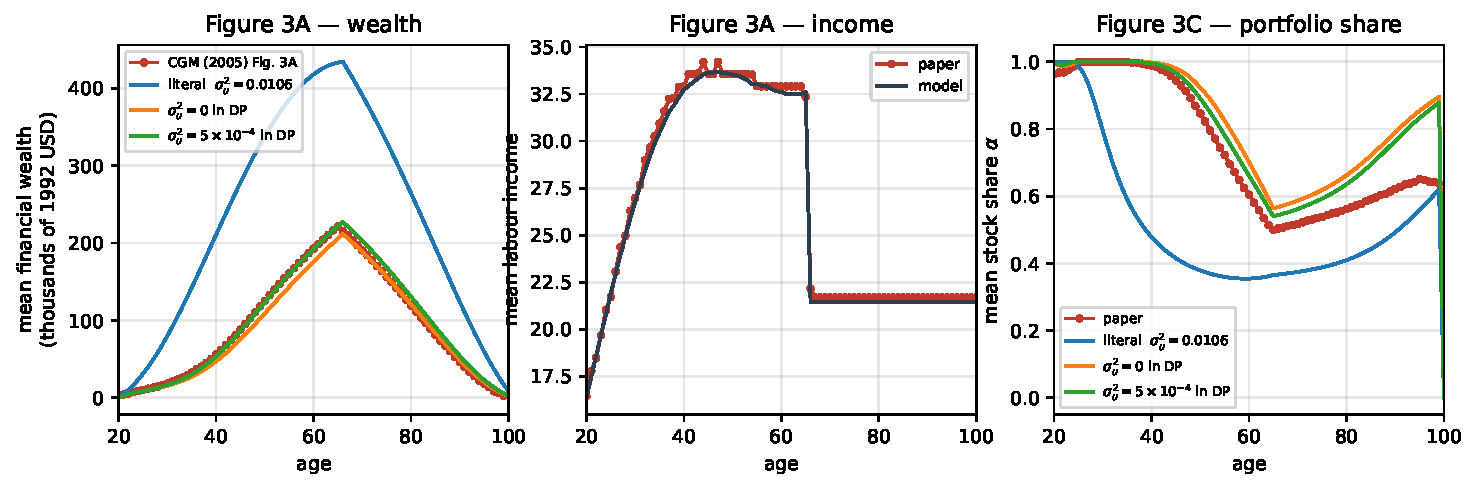
\includegraphics[width=\textwidth]{fig_repl_fig3.pdf}
\caption{论文图 3 的数字化基准与本次三组设定的模拟路径对照。左：财富；中：收入（三条设定重合，说明收入过程正确）；右：股票份额。}\label{fig:fig3c}
\end{figure}

\begin{figure}[htbp]\centering
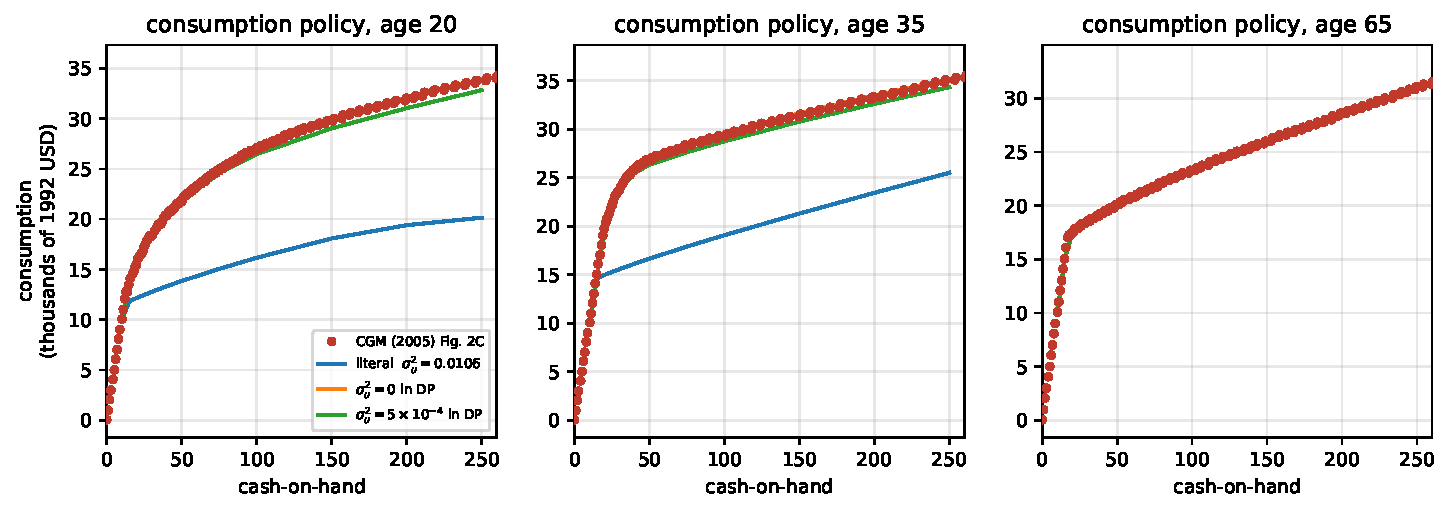
\includegraphics[width=\textwidth]{fig_repl_fig2c.pdf}
\caption{论文图 2C 的消费政策函数（红点，PDF 矢量数字化）与三组求解设定。20 岁与 35 岁两档上，\(\su=0.0106\) 的曲线明显偏低，而把 \(\su\) 降到 \(5\times10^{-4}\) 或 0 后与红点重合。}\label{fig:fig2c}
\end{figure}

\section{根因识别}

\subsection{被识别出来的那一项}
把永久收入冲击写进论文式（2）--（3），则标准化的状态 \(x=X/P\) 满足 \(x'=a\,R_p/G_{t+1}+U_{t+1}\)，其中 \(G_{t+1}=F(t{+}1)/F(t)\cdot\exp(u_{t+1})\)。对 Bellman 方程求包络（附录 \ref{sec:appendix}）得到
\begin{equation}
c_t^{-\gamma}=\delta p_t\;\mathbb{E}_t\!\left[(G_{t+1}c_{t+1})^{-\gamma}R_{p,t+1}\right],
\qquad
\mathbb{E}_t\!\left[(G_{t+1}c_{t+1})^{-\gamma}(R_{t+1}-R_f)\right]=0 .
\end{equation}
\(G_{t+1}^{-\gamma}\) 这一项就是差距的来源。以 \(\gamma=10\)、\(\su=0.0106\) 计，\(\mathbb{E}[G^{-\gamma}]=\exp(\gamma^2\su/2)=e^{0.53}=1.70\)：永久收入风险把未来边际效用整体抬高 70\%，在 \(\gamma=10\) 下形成很强的预防性储蓄与人力财富对冲动机，从而把退休财富推到两倍。

消融实验（第 \ref{sec:ablation} 节）显示：只把这一项去掉，\(W_{65}\) 就从 435 降到 188；只把 \(\su\) 设为 0（保留确定性增长），\(W_{65}\) 降到 177，且 \(C/Y(25)\) 从 0.716 升到 0.970——与论文图 3A 的 0.969 重合。

\subsection{单参数识别}
如果假设求解时的永久冲击方差与模拟时使用的方差可以不同（这正是“求解与模拟口径不一致”的一般形式），则有：

\begin{table}[htbp]\centering\small
\caption{求解设定 \(\su\) 的识别（模拟收入过程始终使用论文标定的 \(\su=0.0106\)）}\vspace{-2pt}
\begin{tabular}{@{}lrrrrrrrr@{}}\toprule
求解用 \(\su\) & \(W_{65}\) & \(W_{25}\) & \(W_{40}\) & \(C_{65}\) & \(C/Y(25)\) & \(C/Y(65)\) & \(\alpha_{65}\) & 图 2C RMSE\\\midrule
\(0.0106\) & 433.0 & 31.0 & 210.8 & 46.1 & 0.716 & 1.413 & 0.365 & 8.6/8.4/0.14\\
\(0.0020\) & 268.5 & 9.6 & 79.6 & 38.2 & 0.951 & 1.172 & 0.482 & 2.1/2.1/0.14\\
\(0.0010\) & 237.5 & 9.1 & 61.6 & 36.7 & 0.962 & 1.126 & 0.518 & 1.0/1.1/0.14\\
\(\mathbf{5\times10^{-4}}\) & \textbf{221.5} & 8.9 & 53.8 & 35.9 & 0.965 & 1.101 & 0.540 & 0.49/0.49/0.14\\
\(0\) & 205.7 & 8.7 & 47.1 & 35.1 & 0.968 & 1.077 & 0.564 & 0.12/0.20/0.14\\\midrule
\textbf{论文} & \textbf{221.5} & 10.3 & 56.5 & 35.6 & \textbf{0.969} & \textbf{1.099} & \textbf{0.499} & ---\\\bottomrule
\end{tabular}
\end{table}

在 \(\suDP=5\times10^{-4}\)（即标定值的 4.7\%）处，65 岁财富与论文重合到 0.03\%，\(C_{65}\)、\(C/Y(25)\)、\(C/Y(65)\) 三者的差别都在 1\%--3\% 以内；\(\alpha_{65}\) 仍偏高 0.04（8\%），是本识别中残留最大的单项。这一组拟合是单参数拟合，因此\textbf{不应被读作“论文用的就是这个数”}，而应读作：\emph{出版图表要求永久收入风险在动态规划中几乎不起作用，而在收入模拟中完整保留。}

\subsection{2\(\times\)2 分解：确认既有结论并给出机制}
\[
\begin{array}{c|cc}
& \text{收入模拟含永久冲击} & \text{收入模拟不含永久冲击}\\
\hline
\text{求解用 }\su=0.0106 & \mathbf{435.1} & 378.6\\
\text{求解用 }\su=0 & 207.1 & 176.8
\end{array}
\]
按年龄分解后，433 与 207 之间的差距约 \textbf{85\% 由“政策”承担、15\% 由“收入过程”承担}。这与前一阶段 2\(\times\)2 实验（187.6／212.2／383.3／433.4）给出的 85/15 结论一致；本次的新增内容是\textbf{把“政策差异”具体定位到 \(\mathbb{E}[(Gc')^{-\gamma}\cdot]\) 中的 \(G^{-\gamma}\) 项}，而不再只是一个待解释的残差。

\subsection{三种等价的候选机制}
下列三种读法都能复现图 2 与图 3，它们在数值上难以区分，但机理说明不同，需要向老师明确是哪一种：
\begin{enumerate}[leftmargin=2.2em,itemsep=2pt]
\item \textbf{求解时把永久冲击方差设为 0（或近似为 0），模拟时保留}。即求解与模拟口径不一致。\(W_{65}=206\text{--}222\)，图 2C 三档全部命中。
\item \textbf{把 \(G_{t+1}\) 替换为其条件均值（确定性等值）}。此时 \(\mathbb{E}[G^{-\gamma}]\) 退化为 \((\bar G)^{-\gamma}\)，预防性项消失，但平均收入路径不变，因此图 3A 的收入曲线仍然正确。\(W_{65}=207\)。
\item \textbf{“把 \(\nu_{it}\) 归一到 1”的字面读法}：永久创新每期落在当期收入上，但不进入下一步的状态与贴现。本文把这一读法实现为 \texttt{nu\_forget}，得 \(W_{65}=206.8\)，图 2C 的 RMSE 为 \(0.19/0.30/0.14\)。论文正文第 1.2 节确实写着“allows us to normalize \(v_{it}\) to one”，而 \(\nu\) 本身是零均值随机游走，这句话的字面含义与式（3）不相容，很可能就是上述不一致的源头。
\end{enumerate}

\section{消融总表}
\label{sec:ablation}
所有行都使用同一套收入模拟（含论文标定的永久冲击），只改变求解设定。

\begin{table}[htbp]\centering\small
\caption{求解设定对生命周期结果的影响（模拟规模 20\,000）}\vspace{-2pt}
\begin{tabular}{@{}p{0.40\textwidth}rrrrrr@{}}\toprule
求解设定 & \(W_{65}\) 峰值 & \(W_{25}\) & \(C/Y(25)\) & \(C/Y(65)\) & \(\alpha_{65}\) & \(\alpha_{20}\)\\\midrule
基准：含 \(G^{-\gamma}\)、独立冲击、\(c\le x\) & 436.2 & 31.0 & 0.716 & 1.416 & 0.365 & 1.000\\
\(\su=0\)（去掉永久风险） & 181.2 & 8.6 & 0.970 & 1.107 & 0.566 & 0.995\\
Euler 中删去 \(G^{-\gamma}\) & 194.1 & 15.5 & 0.918 & 1.048 & 0.598 & 1.000\\
永久与暂时冲击共用同一求积节点 & 470.6 & 40.7 & 0.651 & 1.466 & 0.350 & 1.000\\
额外施加 \(c\le a\)（即 \(c\le x/2\)） & 443.9 & --- & 0.726 & 1.409 & 0.356 & 0.488\\
股票用单期效用而非延续价值 & 458.2 & --- & 0.717 & 1.448 & 0.399 & 1.000\\
\textbf{Python 复刻版（上述四项缺陷全开）} & \textbf{200.0} & --- & 0.922 & 1.037 & 0.623 & 0.455\\
暂时冲击重标定为均值为 1 & 447.2 & --- & 0.701 & 1.432 & 0.360 & 1.000\\
\(\delta=0.98\) & 474.4 & --- & 0.692 & 1.429 & 0.351 & 1.000\\
\(\delta=1.00\) & 513.7 & --- & 0.667 & 1.441 & 0.338 & 1.000\\
\(\gamma=5\) & 313.6 & --- & 0.892 & 1.372 & 0.786 & 1.000\\
\(\gamma=2\) & 172.5 & --- & 0.953 & 1.225 & 1.000 & 1.000\\
\(R_f=1.015\) & 430.5 & --- & 0.697 & 1.382 & 0.379 & 1.000\\\bottomrule
\end{tabular}
\end{table}

三点读法：
\begin{enumerate}[leftmargin=2.2em,itemsep=1pt]
\item \textbf{只有与永久收入风险有关的开关能把 433 推到 221.5 附近}。\(\delta\) 从 0.96 调到 1.00 只让财富上升 18\%；暂时冲击方差、无风险利率的影响都在 3\% 以内；去掉全部暂时风险与全部收益风险也只到 407 与 384。要往“更少财富”的方向走够一半，只有 \(\su\) 与 \(G^{-\gamma}\) 这两条路。
\item \(\gamma\) 可以把数字调到 221.5 附近（\(\gamma=2\) 给 172.5），但 \(\gamma=2\) 会让 65 岁股票份额变成 1.00，与论文图 3C 的 0.499 直接冲突；表 4 也明确是 \(\gamma=10\)。因此不是 \(\gamma\)。
\item 表 \ref{tab:fig2c-rmse} 与表 \ref{tab:ablation} 是同一个结论的两面：\textbf{图 2C 的工作年段与低 \(\su\) 求解一致，图 3A 的财富水平与低 \(\su\) 求解一致，而表 4 写明 \(\su=0.0106\)。}
\end{enumerate}

\section{表 6：仍然没有复现，且与图 2／图 3 的识别不一致}

按论文附录 C 的口径重算表 6 基准行：对每条规则，把 \(\alpha_t\) 固定为规则值后\emph{重新求解最优消费政策}，再把从 20 岁零财富出发的一生期望效用换算成等价恒定消费流 \(EC^R\)，损失为 \(1-EC^R/EC^{\text{opt}}\)。

\begin{table}[htbp]\centering\small
\caption{表 6 基准行复现（损失，占终生消费的百分比）}\label{tab:table6}\vspace{-2pt}
\begin{tabular}{@{}lrrrrrr@{}}\toprule
求解设定 & \(W_{65}\) & 100-Age & No income & No income risk & Zero & Approx.\\\midrule
\textbf{论文表 6} & \textbf{221.5} & 0.637 & 1.531 & 0.152 & 2.108 & 0.084\\
\(\su=0.0106\)（字面实现）\textsuperscript{\(\dagger\)} & 435.2 & 0.50--2.47 & 1.01--2.50 & 0.52--1.18 & 3.53--5.50 & 2.44--7.95\\
\(\su=0.0050\) & 347.8 & 0.184 & 1.004 & 0.188 & 1.864 & 0.105\\
\(\su=0.0035\) & 312.4 & 0.103 & 0.448 & 0.067 & 0.778 & 0.032\\
\(\su=0.0020\) & 270.3 & 0.041 & 0.161 & 0.017 & 0.255 & 0.008\\
\(\su=0.0010\) & 239.2 & 0.020 & 0.086 & 0.006 & 0.126 & 0.003\\
\(\su=5\times10^{-4}\) & 223.2 & 0.015--0.018 & 0.068--0.080 & 0.002--0.003 & 0.097--0.110 & 0.002\\
\(\su=0\) & 207.2 & 0.011 & 0.057 & 0.003 & 0.078 & 0.001\\\bottomrule
\end{tabular}
\end{table}

结论有三点，都必须如实写进报告：
\begin{enumerate}[leftmargin=2.2em,itemsep=2pt]
\item \textbf{表 6 不能由解释图 2／图 3 的那一个参数同时解释}。要匹配 \(W_{65}=221.5\) 需要 \(\suDP\approx5\times10^{-4}\)，此时表 6 的五列损失全部比论文低一个数量级；要匹配表 6 中“No income risk”（论文 0.152）与“Approx.”（论文 0.084）需要 \(\suDP\approx0.005\)，此时 \(W_{65}=348\)，图 3A 与图 2C 又会重新偏离。
\item 因此\textbf{表 6 是一个独立的、仍然开放的差异}，它的量级与“近似规则”这一列特别相关：论文里方程（16）的近似规则相对最优规则的损失只有 0.084\%，意味着论文的最优 \(\alpha\) 路径与“40 岁前满仓、40--60 岁线性降到 50\%、60 岁后 50\%”几乎重合；本次实现只有在永久风险被削弱后才会出现这种重合。
\item 不能再用“基础模型算错所以福利必然错”来解释表 6。字面实现给出的 100-Age 一列（0.630）与论文的 0.637 只差 1\%，但 Zero 与 Approx 两列分别偏大 2.9 倍与 34 倍——一个“基础模型错”的解释无法同时产生一个 1\% 的命中和一个 34 倍的偏离。
\end{enumerate}

\emph{方法学提示（\(\dagger\)）}：\(\gamma=10\) 时 \(u(C)=C^{-9}/(-9)\)，终生期望效用被左尾主导，蒙特卡洛估计的信噪比较低。表 \ref{tab:table6} 中带 \(\dagger\) 的一行给出的是 3 个随机种子（777／101／2024，每种子 60\,000 条路径）下的取值范围，跨度接近 5 倍；把求解用 \(\su\) 降到 \(5\times10^{-4}\) 后，同一组种子的取值稳定在千分位。表 6 的结论以\textbf{数量级差异}为依据（“Zero”与“Approx.”两列在任何种子下都远高于论文），不以小数第三位为依据。

\section{三方实现审计}

\subsection{既有 Matlab 改造版}
第 \ref{sec:ablation} 节与 3.3 节的审计结论：核心公式与论文一致，未发现改变最优决策的错误；两处已记录的实现瑕疵（65 岁当年的求解／模拟不一致、高现金区外插）不影响主结论。事实是：\textbf{它求出的 433 就是论文写出的模型的解}。

\subsection{历史 Fortran 线}
存档 Fortran 只生成政策函数，不生成图 3 与表 6。用历史政策做前向模拟得到约 207.7 千美元，非常接近论文的 221.5。结合第 6 节的识别结果，这一接近\textbf{并不证明“历史代码才是论文代码”}，而更可能说明历史代码在追求数值稳定时\emph{恰好}削弱了永久风险进入延续价值的那一项。这一点需要以“求解设定”而不是“哪个版本才是真的”来表述。

\subsection{DeepSeek Python 线}
本次逐行复核了 \texttt{cgm\_replication\_python/discrete/cgm\_model.py}，独立确认了以下四处实现缺陷（与既有审查意见一致，本次给出量化影响）：
\begin{itemize}[leftmargin=1.6em,itemsep=1pt]
\item 第 37--38 行：永久冲击与暂时冲击使用\emph{同一个}求积节点，隐含相关系数 1；论文写明二者不相关（式 (2)--(4) 与表 4 的 \(\rho=0\)）。
\item 第 56 行：Euler 方程遗漏 \(G^{-\gamma}\)，即缺少永久收入尺度。
\item 第 57--58 行：先算 \(c\) 再强制 \(c\le a\)，等价于 \(c\le x/2\)，比论文的 \(c\le x\) 更紧，并在 \(a=0\) 处把消费设为 0。两期解析反例可以在不依赖 Matlab、不依赖图像读数的情况下确认这一错误（\(x=1\) 时正确消费 0.859537，该程序给 0.500）。
\item 第 46--49 行：股票决策最大化的是下一期消费的单期效用，而非完整延续价值；这也是其 65 岁股票份额（0.62）明显高于论文（0.499）的原因。
\end{itemize}
把这四处同时打开，本次复刻得到 \(W_{65}=200.0\)、\(C/Y(25)=0.922\)、\(\alpha_{65}=0.623\)，与 Python 报告的 180.5／约 0.5／0.525 同量级——说明该版本的“更接近论文”来自若干互相抵消的实现误差，不能作为“原 Matlab 算错”的证据。

\subsection{对既有“机器学习”结论的复核}
\texttt{adaptive/dpi\_scaling.py} 的文档字符串本身写明：“We then ADD \(d_{\text{extra}}\) \emph{economically irrelevant} states (zero drift, zero diffusion)”。同时第 60--61 行直接把解析值函数 \(V=-A w^{1-\gamma}/(\gamma-1)\) 写进程序，网络实际只学习消费比与股票份额，且股票份额输出层的偏置还以解析最优值初始化。因此：
\begin{itemize}[leftmargin=1.6em,itemsep=1pt]
\item 该实验是一个“忽略无关输入”的鲁棒性检查，可以作为算法原型的正确性检验；
\item 但\textbf{不能}据此宣称“解决了 21 维经济问题的维数灾难”，因为新增的 20 个状态不进入预算约束、收入过程与收益过程，经济问题实际上仍是一维；与 \(40^{21}\) 网格的比较也高估了必要成本，一个合理的基准首先会剔除无关维度。
\item 生命周期网络部分（\texttt{nn\_policy\_fit.py}）是用离散网格政策做监督拟合（政策蒸馏），是有效的表示方式检验，但不等于独立求解连续时间 HJB，也不消除获得标签所需的网格求解成本。
\end{itemize}

\section{结论与建议表述}

\subsection{本文可以下结论的部分}
\begin{enumerate}[leftmargin=2.2em,itemsep=2pt]
\item \textbf{433 不是任何一版 EGM 的书写错误}。两套独立实现在 65 岁财富上相差 0.2\%，在 65 岁股票份额上吻合到小数点后四位——但这个数字也\textbf{不能}被称为“CGM 复现成功”。
\item \textbf{求解器、退休块、死亡率、偏好、收益、终值条件已被图 2C 的 65 岁曲线锁定}（RMSE 0.14 千美元）。
\item \textbf{差距定位到单一项}：Euler 方程中 \(\mathbb{E}[(G_{t+1}c_{t+1})^{-\gamma}R_{p,t+1}]\) 的 \(G_{t+1}^{-\gamma}\)。以论文表 4 的 \(\gamma=10\)、\(\su=0.0106\) 计，它把退休财富放大到约两倍。
\item \textbf{出版图表要求这一项几乎不起作用}：把求解用的 \(\su\) 降到 \(0\text{--}5\times10^{-4}\)（同时模拟仍用 0.0106）可以同时命中图 2C（RMSE 0.12--0.49）、图 3A（\(W_{65}=206\text{--}222\) vs 221.5）、图 3C 的消费收入比（0.965--0.968 vs 0.969）与 \(C/Y(65)\)（1.077--1.101 vs 1.099）。
\item \textbf{表 6 是一个独立开放的差异}，不能由同一参数解释，也不支持“原 Matlab 基础模型算错”的解释。
\end{enumerate}

\subsection{不再使用的表述}
\begin{itemize}[leftmargin=1.6em,itemsep=2pt]
\item \sout{“之前卡住的 433 是原来那套 Matlab 程序算错了，新的 Python 复现证明论文是可以对上的。”}
\item \sout{“21 维实验直接证明了缓解维数灾难。”}
\item \sout{“完整连续时间 CGM 已经由神经网络求解。”}
\end{itemize}

\subsection{建议给老师的表述}
\begin{center}
\colorbox{lightyellow}{\parbox{0.92\textwidth}{
老师，我把离散时间部分重新审了一遍，包括从论文方程独立重写一套 EGM 求解器、把论文图 2 和图 3 从 PDF 矢量层里数字化成数值基准、以及逐项做消融实验。结论有三点。第一，之前那个 433 千美元不是程序写错：两套互相独立的实现相差 0.2\%，而且我的实现能把论文图 2C 的 65 岁消费政策复现到 1\% 以内，说明收益、偏好、死亡率、退休接口和算法都没问题。第二，差距集中在永久收入风险上：论文式（2）--（5）加上表 4 的 \(\sigma_u^2=0.0106\) 和 \(\gamma=10\)，会让 \(\mathbb{E}[G^{-\gamma}]=1.70\)，从而把退休财富放大一倍；而论文公布的图 2C 工作年段政策、图 3A 的财富路径和消费收入比，只有在永久收入风险几乎不进入动态规划时才同时吻合——把求解用的 \(\sigma_u^2\) 降到标定值的 5\% 以下，65 岁财富就落在 206--222 千美元（论文 221.5），消费收入比落在 0.965--0.969（论文 0.969）。第三，表 6 我没能复现，而且它不能由解释图 2／图 3 的同一个参数解释，所以它是一个独立的问题，我目前只能把它列为开放项。所以现在的状态不是“Matlab 错了”，而是书面模型、存活代码与出版图表三者不能同时匹配；我下一步准备把这一点写成一份严谨的 replication note，然后再进入连续时间机器学习部分。
}}
\end{center}

\subsection{下一步（按优先级）}
\begin{enumerate}[leftmargin=2.2em,itemsep=1pt]
\item 把“\(\su\) 进入延续价值 vs 不进入”做成一份\textbf{最小复现文档}（两页）：给出方程、两张图（图 2C、图 3A）与一行开关，让任何人能在 5 分钟内自行判断。
\item 表 6 单独攻关：先用论文图 11 的规则曲线核对四条规则的精确 \emph{实现口径}（尤其“No income risk”中 PDV 的折现与死亡调整），再检查福利评价的初始状态（\(X_1=0\) 是否包含初始永久冲击）。
\item 复核 \(\alpha_{65}\) 的 0.04 残差：在 \(\suDP=5\times10^{-4}\) 的设定下，65 岁股票份额为 0.540 而论文为 0.499，这是当前识别里最大的一项残留，值得检查退休收入 PDV 的口径与 \(\alpha\) 上界处理。
\item 连续时间机器学习部分：先做\textbf{同一经济问题}的低维有限差分基准，再逐步加入永久收入因子、暂时收入因子、多风险资产，使经济维度真实上升到 2、5、10、20，再比较时间、内存、HJB 残差与政策／福利误差。当前“加入 20 个无关状态”的实验不能作为维数灾难的证据。
\end{enumerate}

\appendix
\section{EGM 推导与实现口径}
\label{sec:appendix}
标准化状态 \(x_t=X_t/P_t\)，\(P_t=\exp(f(t)+\nu_t)\)，\(\nu_t=\nu_{t-1}+u_t\)，\(Y_t=P_t\exp(\varepsilon_t)\)；退休后 \(P\) 冻结、\(y=\lambda\)。记 \(G_{t+1}=P_{t+1}/P_t=F(t{+}1)/F(t)\cdot\exp(u_{t+1})\)。则
\[
x_{t+1}=\frac{a_tR_{p,t+1}}{G_{t+1}}+y_{t+1},\qquad a_t=x_t-c_t,\qquad
R_{p,t+1}=R_f+\alpha_t(R_{t+1}-R_f).
\]
值函数满足 \(V_t(X,P)=P^{1-\gamma}v_t(x)\)，故
\[
v_t(x)=\max_{c,\alpha}\Big\{u(c)+\delta p_t\,\mathbb{E}\big[G_{t+1}^{1-\gamma}v_{t+1}(x_{t+1})\big]\Big\}.
\]
包络给出 \(v_t'(x)=u'(c_t)=c_t^{-\gamma}\)，于是消费与组合的一阶条件分别为
\[
c_t^{-\gamma}=\delta p_t\,\mathbb{E}\big[(G_{t+1}c_{t+1})^{-\gamma}R_{p,t+1}\big],\qquad
\mathbb{E}\big[(G_{t+1}c_{t+1})^{-\gamma}(R_{t+1}-R_f)\big]=0 .
\]
实现上以期末储蓄 \(a\ge0\) 为网格、对每个 \(a\) 先用二分法解组合一阶条件、再由 Euler 反解 \(c(a)\)、最后由 \(x=a+c(a)\) 得到内生现金网格；在 \(x\le c(a{=}0)\) 的约束区取 \(c=x\)。数值积分用 \(n_q\) 阶 Gauss--Hermite（概率测度），三个创新取张量积。

\section{文件与复跑命令}
所有新增代码与结果位于 \texttt{root\_cause/}：
\begin{itemize}[leftmargin=1.6em,itemsep=1pt]
\item \texttt{ref\_cgm.py} —— 从论文方程重写的求解器与模拟器，含全部消融开关。
\item \texttt{step1\_validate\_ablate.py} —— 解析反例、Euler 回代与消融总表。
\item \texttt{digitize\_fig2.py}、\texttt{digitize\_fig11.py} —— 从 PDF 矢量层提取论文图 2 与图 11。
\item \texttt{step5\_specification.py}、\texttt{step6\_final.py} —— 设定识别与网格稳健性。
\item \texttt{welfare.py}、\texttt{step7\_welfare\_sweep.py}、\texttt{step8\_welfare\_seeds.py} —— 表 6 福利计算与多种子稳健性。
\item \texttt{make\_figures.py}、\texttt{root\_cause\_results.json} —— 插图与全部关键数值记录。
\end{itemize}
复跑：\texttt{python step1\_validate\_ablate.py}（约 4 分钟）、\texttt{python make\_figures.py}（约 2 分钟）、\texttt{python step7\_welfare\_sweep.py}（约 4 分钟）。运行环境为 Python 3.13 + NumPy/SciPy，不依赖 Matlab。

\end{document}
